\chapter[APÊNDICE \ref{Ap:SLR}]{Problema de \textit{Scordelis-Lo roof}}
\label{Ap:SLR}

O primeiro exemplo simulado trata-se de um problema comumente encontrado para problemas de cascas, denominado de \textit{Scordelis-Lo roof}, conforme ilustrado na Figura \ref{fig:scordelis}. Esse exemplo se caracteriza por uma cobertura curva sujeita a um carregamento gravitacional $q$, distribuído por unidade de área, na direção $x_3$ para baixo. Os parâmetros geométricos são dados por: comprimento $L=50$, raio de curvatura $R=25$, espessura $t=0,25$ e ângulo $\theta=40^\circ$. O valor da carga aplicada é $q=90$. O material que constitui a cobertura possui módulo de Young $E=4,32\times10^8$ e Poisson nulo. As extremidades estão presas por um diafragma rígido ($u_1=u_3=0$). Os resultados são comparados com os obtidos por \citeonline{BELYTSCHKO1985221,ZHOU2022108568,CHAUDINH2023110222}, os quais apontam que o deslocamento vertical do nó $A$ é de 0,3024.

\begin{figure}[h!]
    \centering
    \caption{Problema de \textit{Scordelis-Lo roof}.}
    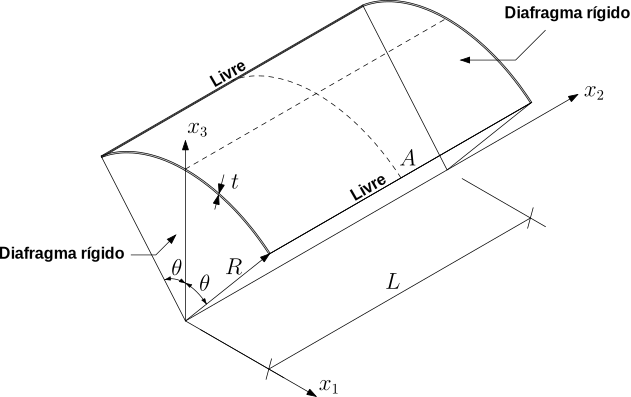
\includegraphics[width=0.75\linewidth]{Figuras/scordelis/scordelis_lo.pdf}
    \\Fonte: Autoria Própria (\the\year).
    \label{fig:scordelis}
\end{figure}

Para a simulação do problema aproveitou-se da simetria da cobertura, o que possibilitou a modelagem de apenas um quarto do problema. Assim utilizou-se uma malha estruturada com orientação à esquerda contendo 552 elementos triangulares de aproximação quadrática, resultando em 7987 graus de liberdade. A malha é apresentada na Figura \ref{fig:scordelis-mesh}. As faces laterais observadas na malha foram criadas por conta da forma de construção da aresta circular da cobertura, sendo atribuídos $E=\nu=0$ para os elementos dessas faces. O problema foi considerado em pequenos deslocamentos e deformações, ou seja, utilizou-se somente uma iteração de Newton-Raphson.

\begin{figure}[h!]
    \centering
    \caption{Malha utilizada na simulação de \textit{Scordelis-Lo roof}.}
    \begin{subfigure}{0.35\textwidth}
        \includegraphics[width=\linewidth]{Figuras/scordelis/malha1.png}
        \caption{Perspectiva isométrica.}
    \end{subfigure}
    \begin{subfigure}{0.35\textwidth}
        \includegraphics[width=\linewidth]{Figuras/scordelis/malha2.png}
        \caption{Vista superior.}
    \end{subfigure}
    \\Fonte: Autoria Própria (\the\year).
    \label{fig:scordelis-mesh}
\end{figure}

Dessa forma, chegou-se a um deslocamento de 0,3008 nos cálculos realizados, representando um desvio de 0,5291\% em relação à referência. A Figura \ref{fig:scordelis-displ} apresenta o campo de deslocamentos obtido para um quadrante da cobertura.

\begin{figure}[h!]
    \centering
    \caption{Campos de deslocamentos obtido na simulação de \textit{Scordelis-Lo roof}.}
    \begin{subfigure}{0.05\textwidth}
        \includegraphics[width=\linewidth]{Figuras/scordelis/eixos.png}
    \end{subfigure}
    \begin{subfigure}{0.31\textwidth}
        \includegraphics[width=\linewidth]{Figuras/scordelis/ux.png}
    \end{subfigure}
    \begin{subfigure}{0.31\textwidth}
        \includegraphics[width=\linewidth]{Figuras/scordelis/uy.png}
    \end{subfigure}
    \begin{subfigure}{0.31\textwidth}
        \includegraphics[width=\linewidth]{Figuras/scordelis/uz.png}
    \end{subfigure}
    \\Fonte: Autoria Própria (\the\year).
    \label{fig:scordelis-displ}
\end{figure}

Assim, observa-se que tais campos estão muito semelhantes aos apresentados por \citeonline{ZHOU2022108568}, sendo satisfatoriamente verificada a análise realizada.

Também realizou-se uma análise quanto à convergência da malha, onde dividiu-se as arestas do problema em $N$ partes. A Tabela \ref{tab:scordelis-sol} apresenta os resultados obtidos, sendo os valores do deslocamento em função do refinamento da malha ilustrados na Figura \ref{fig:shell-static-sol}.

\begin{table}[h!]
    \centering
    \caption{Análise da convergência da malha para o problema de \textit{Scordelis-Lo roof}.}
    \begin{tabular}{ccccc}
        \hline
        $N$ & Número de elementos & Graus de liberdade & Calculado & Desvio relativo \\\hline
        5   & 64                  & 1001               & 0,2115    & -30,060\%       \\
        6   & 88                  & 1351               & 0,2361    & -21,925\%       \\
        7   & 11                  & 1757               & 0,2638    & -12,765\%       \\
        8   & 148                 & 2219               & 0,2726    & -9,854\%        \\
        9   & 184                 & 2737               & 0,2824    & -6,614\%        \\
        10  & 224                 & 3311               & 0,2863    & -5,324\%        \\
        11  & 268                 & 3941               & 0,2893    & -4,332\%        \\
        12  & 316                 & 4627               & 0,2925    & -3,274\%        \\
        13  & 368                 & 5369               & 0,2954    & -2,325\%        \\
        14  & 424                 & 6167               & 0,2970    & -1,786\%        \\
        15  & 484                 & 7021               & 0,2978    & -1,521\%        \\
        16  & 552                 & 7987               & 0,3008    & -0,529\%        \\\hline
    \end{tabular}
    \\Fonte:Autoria Própria (\the\year).
    \label{tab:scordelis-sol}
\end{table}

\begin{figure}[h!]
    \centering
    \caption{Deslocamento vertical do ponto $A$ para diferentes malhas.}
    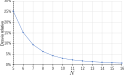
\includegraphics[width=0.75\linewidth]{Figuras/scordelis/static-sol.pdf}
    \\Fonte: Autoria Própria (\the\year).
    \label{fig:shell-static-sol}
\end{figure}

Igualmente analisou-se o resultado com aquele obtido pelo \textit{software} ANSYS, o qual retornou um deslocamento de 0,3020. Assim o desvio relativo do resultado calculado com o do ANSYS é de 0,3973\%. Além disso, observou-se os deslocamentos verticais ao longo da aresta livre da cobertura, os quais são apresentados na Figura \ref{fig:scordelis-graph}.

\begin{figure}[h!]
    \centering
    \caption{Deslocamento vertical ao longo da aresta livre da cobertura.}
    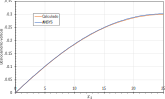
\includegraphics[width=0.7\linewidth]{Figuras/scordelis/deslocamento.pdf}
    \\Fonte: Autoria Própria (\the\year).
    \label{fig:scordelis-graph}
\end{figure}